%Documento di proprietà di Vito Stefano Birardi™
%Qui sono presenti i package più comuni che usi, ricorda di usare solo quelli che ti servono 

%Variabili comuni
\newcommand{\Titolo}{Progetto A\_Clus - Documentazione}
\newcommand{\Data}{\today}
\newcommand{\Materia}{}

%Comandi troppo lunghi da scrivere possono essere ri-operazionalizzati qui

\newcommand{\image}[3]{%
    \begin{figure}[h!]
    \centering
    \includegraphics[width = 0.5 \textwidth]{#1}
    \caption{#2}
    \label{#3}%
\end{figure}}

%Package per la formattazione del foglio

\documentclass[a4paper]{article}
\usepackage{amsmath}
\usepackage{amssymb}

%Package per la lingua dei capitoli

\usepackage[italian]{babel}

%Package per intestazione e pié di pagina

\usepackage{fancyvrb}
\usepackage{fancyhdr, lastpage}

%Package aggiuntivi 

\usepackage{cancel}
\usepackage{etoolbox}
\usepackage{xcolor}
\usepackage{subfig}
\usepackage{tikz, lmodern}
\usepackage[most]{tcolorbox}
\usepackage{graphicx}
\usepackage{parskip}
\usepackage{multicol}
\pagestyle{fancy}

%Formattazione di intestazione e pié di pagina


\lhead{\Data}
\rhead{Vito Stefano Birardi}
\lfoot{\Materia}
\rfoot{Pagina \thepage\ di \pageref{LastPage}}
\renewcommand{\footrulewidth}{0.5pt}
\fancyfoot[C]{}
\patchcmd{\chapter}{\thispagestyle{plain}}{\thispagestyle{fancy}}{}

%Preambolo per prima pagina

\title{\Titolo}
\author{
    A cura di: 
    Vito Stefano \\ Lorenzo Gelao
}
\date{\Data}

%Inizio documento vero e proprio


\begin{document}
\maketitle
\newpage
\tableofcontents
\newpage

\section{Introduzione}

Il progetto in questione verte sull'argoemento dell'\textit{Agglomerative Clustering}, una tecnica di clusterizzazione basata sui metodi Signle distance e Average Distance. 

Il progtto in questione è suddiviso in una parte client e una server, che comunicando tra loro, generano il dendrogramma, permettendo inoltre di visualizzare e memorizzare tali risultati o di caricarne dei precedenti.

È inoltre possibile visualizzare nuovamente dei file caricati in passato per visualizzare i cluster e i dendrogrammi associati. 


\subsection{Agglomerative Clustering}

L'algoritmo di clustering utilizzato in tale progetto, come si può desumer dal nome, sfrutta il concetto di clustering agglomerativo. In pratica, tratta ciascun cluster in maneira separata dagli altri, unendo progressivamente quelli più vicini, in base a due crtieri principali, nel nostro caso.

Il princiaple vantaggio  rispetto ad altri algoritmi di lcustering, come il k-means, è che in questo modo non è necessario speficiare in anticippo la quantità di cluster da analizzare. 

I criteri utilizzati nel progetto A-CLus sono i seguenti: 

\begin{enumerate}
    \item \textbf{Single-Link}: tale criterio determina la distanza minima tra i punti dei vari cluster

    \begin{equation}
        D\left(C1,C2\right) = \underset{\left(t1 \in C1,t2 \in C2\right)}{min}\left( dist\left(t1,t2\right)\right)
    \end{equation}
\end{enumerate}


Durante l'anno accademico 2024/2025, l'oggetto di ricerca è stato incretrato su "A-CLus", una piattaforma con architettura client-server dedicata all'analisi dei dati mediante algoritmi di clustering gerarchico agglomerativo. La componente server esegue le operazioni di clustering impiegando le metodologie Single Link o Average Link per il calcolo delle distanze inter-cluster e la successiva costruzione del dendrogramma. L'applicativo client, implementato in linguaggio Java, offre agli utenti diverse funzionalità: il caricamento o la creazione di istanze HierarchicalClusterMiner, la rappresentazione grafica del dendrogramma e l'archiviazione dei risultati per analisi successive. È inoltre disponibile la funzione di importazione di file precedentemente salvati, consentendo agli utenti di riesaminare i cluster e i relativi dendrogrammi. 

\subsubsection{Framework Analitico}

La tecnica di clustering agglomerativo implementata nel sistema "A-CLus" costituisce una metodologia avanzata per l'identificazione di \underline{correlazioni latenti nei dataset}. 

Diversamente da tecniche alternative come il k-means, l'approccio agglomerativo elimina la necessità di predefinire il numero di raggruppamenti. La procedura inizializza ciascun elemento come cluster individuale e procede con l'unificazione sequenziale dei cluster con maggiore affinità, applicando metodologie quali:  



Con il procedere delle aggregazioni tra cluster, si sviluppa un dendrogramma che illustra la gerarchia delle aggregazioni. Il procedimento continua fino al raggiungimento di un cluster unificato o fino a una soglia di profondità stabilita dall'utilizzatore. La visualizzazione mediante dendrogramma rende la metodologia particolarmente comprensibile, facilitando l'esplorazione strutturale dei dati a diversi livelli di granularità. Inoltre, questa strategia non è influenzata dalla configurazione iniziale dei centroidi, riducendo così la probabilità di risultati inconsistenti e garantendo una rappresentazione più accurata dell'organizzazione interna del dataset.RiprovaClaude può commettere errori. Verifica sempre le risposte con attenzione.



\section{Guida all'installazione}

Prima di essere in grado di eseguire il programma, è necessario eseguire il file \texttt{risorse.bat} contenuto nella cartella Risorse. 


Una volta eseguito il file, si aprirà una pagina ti Powershell e seguirà un download.

\begin{figure}[h!]
    \centering
    
\includegraphics[width= 0.5\textwidth]{images/nuova docs.png}
    \caption{Schermatta di download}
\end{figure}

Al termine del download del file compresso delle risorse, verranno estratti i file necessari per l'esecuzione del programma.



Per il progetto in questione è necessario installare il Java Developer Kit (JDK) nella versione 22.0.1 e il software di gestione del database MySQL nella sua versione 8.0.39. 

La prima scheda di installazione che apparirà è quella del JDK. 

Verrà chiesto se si vuole eseguire l'installazione del JDK tramite permessi di amministratore, cliccare su \underline{Sì}.

\subsection{Installazione JDK}

Una volta confermata l'esecuzione come amministratore, si procederà all'installazione del JDK.

\begin{figure}[h!]
    \centering
    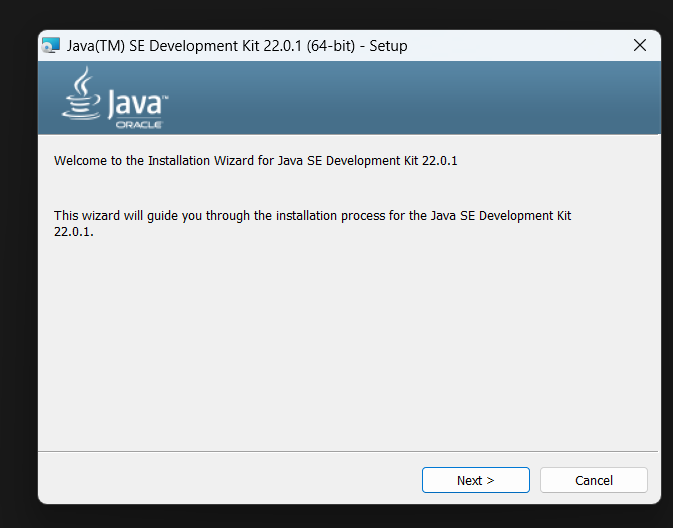
\includegraphics[width= 0.5\textwidth]{images/installazione java.png}
\end{figure}

Cliccare su \textbf{Avanti},nuovamente \textbf{Avanti} e infine, nel caso in cui l'installazione sia andata a buon fine, si dovràò cliccare sul tasto \textbf{Chiudi}.

Una volta completata l'installazione del JDK, si procederà automaticamente con l'installazione del MySQL.

\subsection{Installazione MySQL}

Anche qui sarà necessario fornire i permessi di amministratore, cliccare dunque su \underline{Sì}.

Dopodiché si aprirà la schermata di installazione di MySQL.

\begin{figure}[h!]
    \centering
    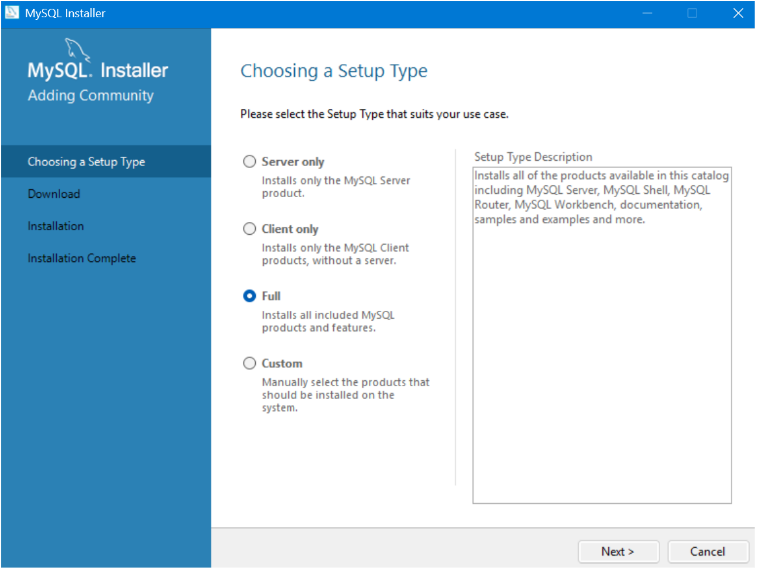
\includegraphics[width= 0.5\textwidth]{images/inizio mysql.png}
    \caption{Scelta del setup}
\end{figure}

Selezionare il tipo di setup \textbf{Full} e cliccare su \textbf{Next}. Tale scelta permetterà di installare tutti i componenti necessari per l'esecuzione del programma.

Si passerà alla schermata di download dei file necessari per l'installazione, cliccare su \textbf{Execute}. 

Tale schermata potrebbe richiedere un po' di tempo per il download dei file, a seconda della velocità della connessione internet. 

Dopo aver scaricato i file, si dovrà cliccare nuovamente su \textbf{Execute}.

\begin{figure}[h!]
    \centering
    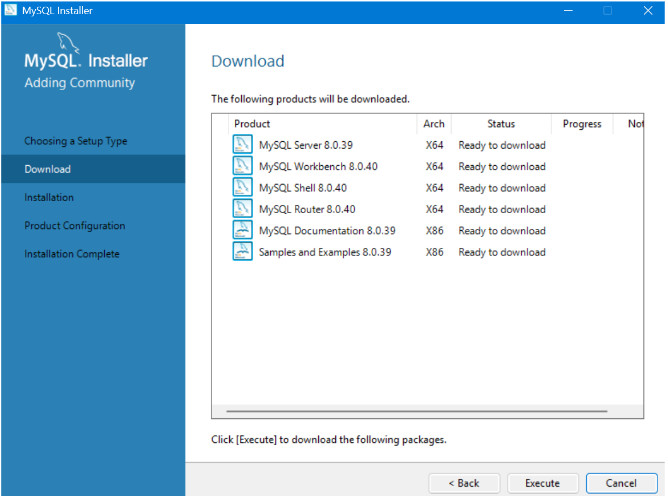
\includegraphics[width= 0.6\textwidth]{images/eexecute.png}
    \caption{Download MySQL}
\end{figure}

Una volta terminato il download, si procederà con la configurazione dell'account MySQL. Si dovrà quindi scegliere una password, necessaria per accedere al database. 


\begin{figure}[h!]
    \centering
    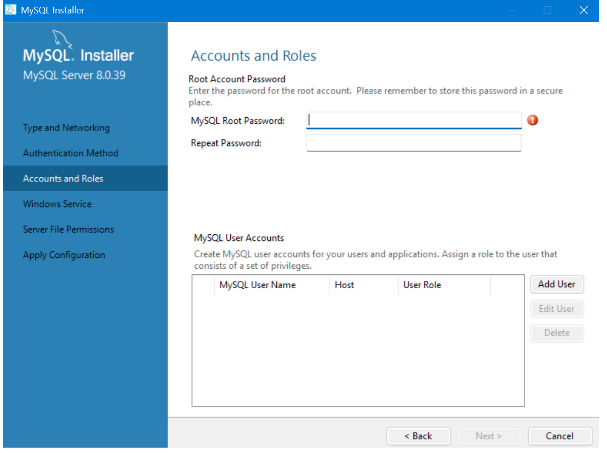
\includegraphics[width= 0.5\textwidth]{images/setup vero e proio musql.png}
    \caption{Configurazione account MySQL}
\end{figure}

Si giungerà infine alla scehermata di applicazione della configurazione del database. Cliccare su \textbf{Execute} per applicare la configurazione.

\begin{figure}[h!]
    \centering
    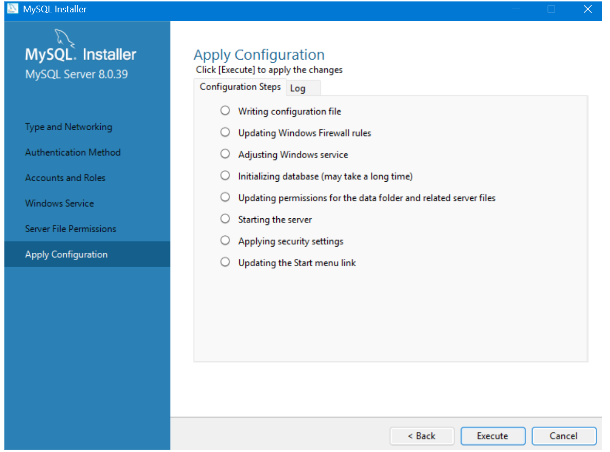
\includegraphics[width= 0.5\textwidth]{images/completamenot.png}
    \caption{Completamento installazione}
\end{figure}


\begin{figure}[h!]
    \centering
    
\includegraphics[width= 0.6\textwidth]{images/insytllazione compeltata.png}
    \caption{Completamento installazione}
\end{figure}

\section{Eseguire A-CLus Base}

\subsection{Operazioni preliminari}

Prima di poter eseguire il programma, occorre importare il database di A-CLus in MySQL. 

Tale file è presente nella cartella \texttt{A-CLus/Risorse} e si chiama \texttt{mapdb.sql}. 

Per importare il database, è necessario semplciemente accedere al MySQL tramite root e digitare il seguente comando \texttt{source} seguito dal percorso del file \texttt{mapdb.sql}. 

Tale percorso si può ottenere semplicemente trascinando il file del database sul terminale di MySQL.

Alle fine dell'importazione, il terminale di MySQL dovrebbe mostrare un messaggio simile al seguente:

\begin{figure}[h!]
    \centering
    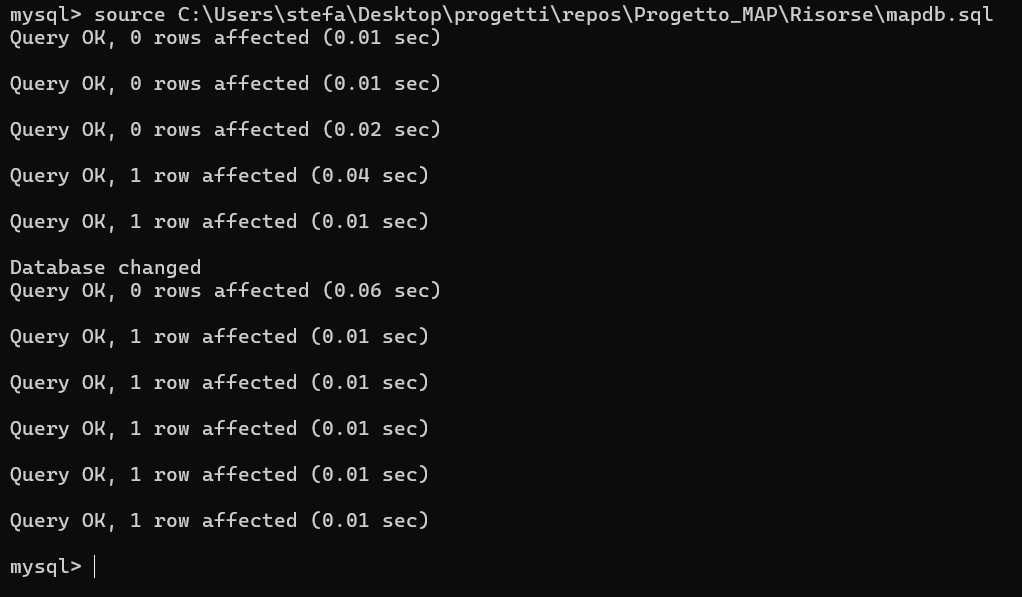
\includegraphics[width=0.5\textwidth]{images/import mysql.png}
\end{figure}

È possibile verificare la corretta importazione anche uscendo da MySQl e accedere con le credenziali dell'utente MapUser, come mostrato nella figura seguente:

\begin{figure}[h!]
    \centering
    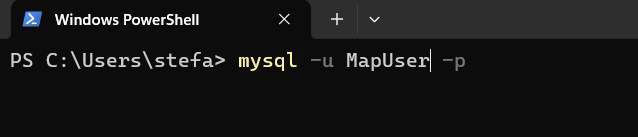
\includegraphics[width=0.5\textwidth]{images/import mapdb.png}
\end{figure}

La password dell'utente MapUser è \texttt{map}. Se viene confermato l'accesso al database, significa che l'importazione è avvenuta con successo. 

\subsection{Avvio dell'applicazione}

Per inizializzare correttamente la versione standard di A-CLus, attenersi alla seguente sequenza operativa:


\begin{enumerate}
    \item Accedere alla directory \texttt{A-CLus\_Base/Bat}
    \item Eseguire il file \texttt{Start\_Server.bat} facendo un doppio click su di esso, assicurandosi che venga mostrato il seguente messaggio a finestra
    
    \begin{figure}[h!]
        \centering
        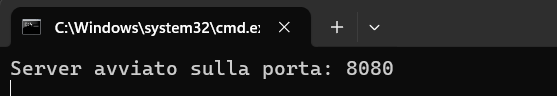
\includegraphics[width=0.5\textwidth]{images/server in esecuzione.png}
    \end{figure}

    \item Dopo aver verificato il corretto funzionamento del server, eseguire il file \texttt{Start\_Client.bat} facendo un doppio click su di esso; se non ci sono problemi con il server, apparirà la seguente schermata:
    
    \begin{figure}[h!]
        \centering
        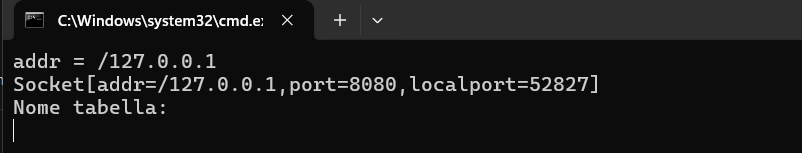
\includegraphics[width=0.5\textwidth]{images/client in esecuzione.png}
        
    \end{figure}
    
\end{enumerate}

\begin{tcolorbox}[colback=white, colframe=gray, title=Avvertenza]
    È necessario mantenere attivo il terminale del server per garantire la comunicazione tra le componenti client e server.
\end{tcolorbox}

\subsection{Avvio dell'ambiente di sviluppo}

Per aprire correttamente il codice sorgente di A-CLus, è necessario seguire le seguenti operazioni nell'ordine in cui sono presentate:

\begin{enumerate}
    \item Aprire la cartella del progetto \texttt{A-Clus\_base}
    \item Incorporare nelle librerie del progetto \texttt{Server} il file \texttt{mySQL\_connector.jar} presente nella cartella \texttt{A-CLus/Risorse}. Nel caso si stia eseguendo il progetto in Visual Studio Code, è possibile eseguire i seguenti passaggi:
    \begin{enumerate}
        \item Aprire il progetto \texttt{A-Clus\_Base}
        \item Recarsi nella sezione \texttt{Referenced Libraries}, in asso a sinistra
        \item Posizionare il cursore sulla cartella e selezionare \texttt{Add JAR/Folder Classpath}, che apparirà sulla destra
        \begin{figure}[h!]
            \centering
            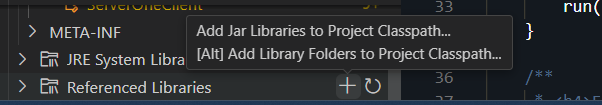
\includegraphics[width=0.5\textwidth]{images/refenereziare il jdbc.png}
        \end{figure}
    \end{enumerate}
    \item Avviare \texttt{MultiServer.java}
    \item Controllare che il server sia in esecuzione correttamente
    \item Aprire il progetto \texttt{MainTest.java} presente nella cartella \texttt{A-CLus\_Base/Client}
\end{enumerate}

\subsection{Interfaccia iniziale}

L'interfaccia iniziale di A-CLus è composta da tre sezioni principali:

\begin{figure}[h!]
    \centering
    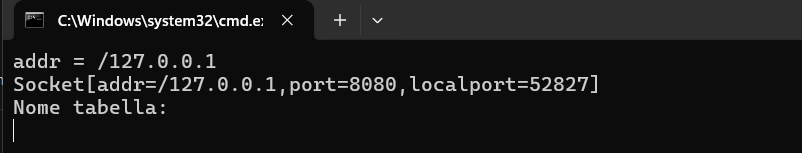
\includegraphics[width=\textwidth]{images/client in esecuzione.png}
    \caption{Interfaccia iniziale di A-CLus}
\end{figure}

L'interfaccia iniziale di A-CLus è composta da tre sezioni principali:

\begin{figure}[h!]
    \centering
    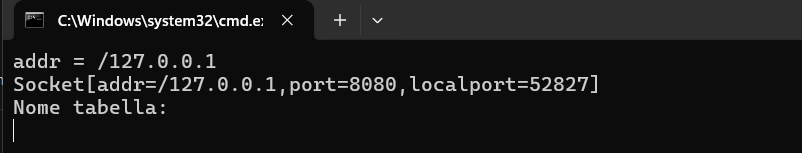
\includegraphics[width=\textwidth]{images/client in esecuzione.png}
    \caption{Interfaccia iniziale di A-CLus}
\end{figure}

\subsection{Selezione delle operazioni disponibili}

\begin{figure}[h!]
    \centering
    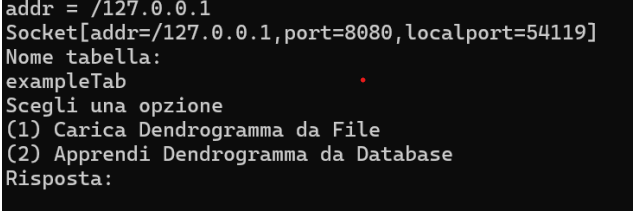
\includegraphics[width=\textwidth]{images/inserimento_tabella.png}
\end{figure}

Dopo l'inserimento della tabella, verrà proposto un menu con due alternative:
\begin{enumerate}
    \item \textbf{Carica Dendrogramma da File}: permette di importare un dendrogramma precedentemente memorizzato
    \item \textbf{Apprendi Dendrogramma da Database}: consente di generare un nuovo dendrogramma analizzando i dati presenti nella tabella selezionata
\end{enumerate}

\subsection{Percorso operativo - Opzione 2 (Generazione nuovo dendrogramma)}

\begin{figure}[h!]
    \centering
    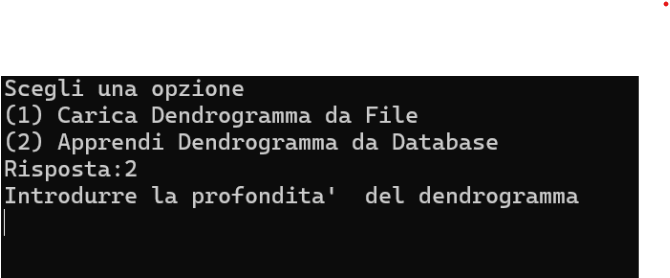
\includegraphics[width=\textwidth]{images/apprendi_datagramma.png}
\end{figure}

Selezionando l'opzione 2, il sistema richiederà l'inserimento del parametro di profondità desiderato per il dendrogramma.

\subsection{Inserimento Profondità}

\begin{figure}[h!]
    \centering
    \includegraphics[width=\textwidth]{images/inserimento_profondità.png}
\end{figure}

Successivamente, l'applicazione proporrà due metodologie di calcolo alternative:
\begin{enumerate}
    \item \textbf{Single-link}: identifica la distanza minima tra cluster, connettendo gli elementi più prossimi tra i gruppi
    \item \textbf{Average-link}: determina la distanza utilizzando la media tra tutti gli elementi dei cluster considerati
\end{enumerate}

\subsubsection{Elaborazione con Single-link}

\begin{figure}[h!]
    \centering
    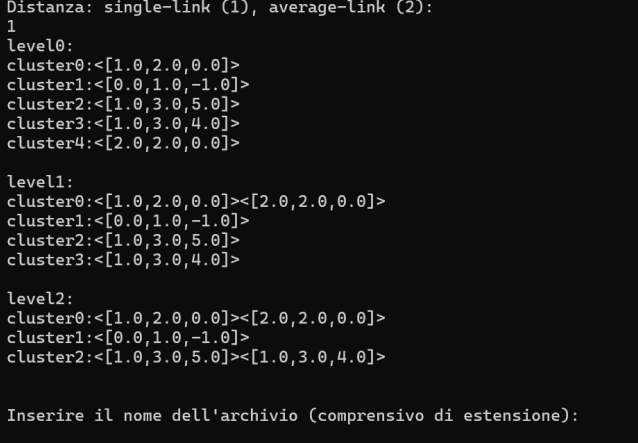
\includegraphics[width=\textwidth]{images/scelta_singleLink.png}
\end{figure}

Selezionando l'opzione Single-link (1), verrà elaborato e visualizzato il dendrogramma risultante. L'applicativo richiederà poi di specificare il nome del file per l'archiviazione del dendrogramma, completo di estensione.

\subsection{Inserimento nome file}

\begin{figure}[h!]
    \centering
    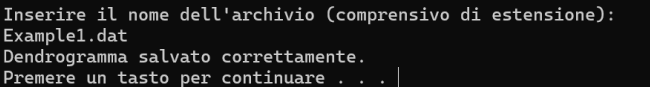
\includegraphics[width=\textwidth]{images/inserimento_nome_file.png}
\end{figure}

Indicare il nome desiderato (esempio: \texttt{Example1.dat}). Il dendrogramma verrà salvato nella cartella \texttt{"saved"} all'interno della directory \texttt{"Jar + Bat"} e l'applicazione terminerà l'esecuzione.

\subsubsection{Elaborazione con Average-link}

\begin{figure}[h!]
    \centering
    \includegraphics[width=\textwidth]{images/scelta_averageLink.png}
\end{figure}

Selezionando l'opzione Average-link (2), il sistema elaborerà il dendrogramma utilizzando il criterio della distanza media e lo visualizzerà a schermo. Successivamente, verrà richiesto di specificare il nome del file per la memorizzazione del dendrogramma, completo di estensione.

\subsection{Percorso operativo - Opzione 1 (Caricamento dendrogramma esistente)}
\begin{figure}[h!]
    \centering
    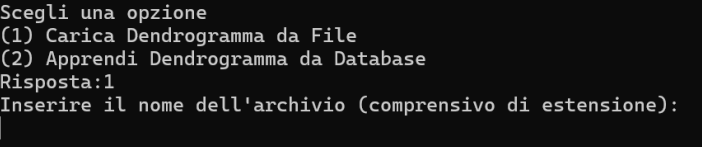
\includegraphics[width=\textwidth]{images/carica_dendrogramma_file.png}
\end{figure}

Selezionando l'opzione 1 per importare un dendrogramma preesistente, sarà necessario indicare il nome completo del file archivio, comprensivo di estensione. I file precedentemente salvati sono localizzati nella cartella \texttt{"saved"} all'interno della directory \texttt{"Jar + Bat"}.

\subsection{Inserimento nome archivio con estensione}

\begin{figure}[h!]
    \centering
    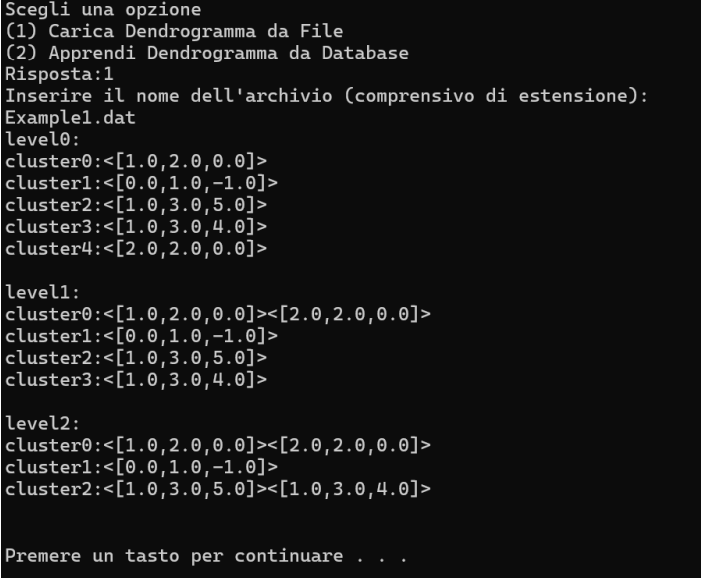
\includegraphics[width=\textwidth]{images/inserimento_nome_archivio.png}
\end{figure}

Dopo l'inserimento del nome dell'archivio, il sistema visualizzerà il dendrogramma caricato e concluderà l'esecuzione.


\end{document}